\documentclass[a4paper,12pt]{article}

\usepackage[slovene]{babel}
\usepackage{amsfonts,amssymb,amsmath}
\usepackage[utf8]{inputenc}
\usepackage[T1]{fontenc}
\usepackage{lmodern}
\usepackage{graphicx}
\usepackage{caption}
\usepackage{subcaption}
\usepackage{float}

\usepackage{url}
\usepackage{icomma}


\def\N{\mathbb{N}} % mnozica naravnih stevil
\def\Z{\mathbb{Z}} % mnozica celih stevil
\def\Q{\mathbb{Q}} % mnozica racionalnih stevil
\def\R{\mathbb{R}} % mnozica realnih stevil
\def\C{\mathbb{C}} % mnozica kompleksnih stevil
\newcommand{\geslo}[2]{\noindent\textbf{#1} \quad \hangindent=1cm #2\\[-1pc]}

\def\qed{$\hfill\Box$}   % konec dokaza
\def\qedm{\qquad\Box}   % konec dokaza v matematičnem načinu
\newtheorem{izrek}{Izrek}
\newtheorem{trditev}{Trditev}
\newtheorem{posledica}{Posledica}
\newtheorem{lema}{Lema}
\newtheorem{opomba}{Opomba}
\newtheorem{definicija}{Definicija}
\newtheorem{zgled}{Zgled}

\title{Problem N teles}
\author{Gaja Jamnik \\
Fakulteta za matematiko in fiziko \\
Oddelek za matematiko}
\date{26.\ oktober 2022}

\begin{document}

%%%%%%%%%%%%%%%%%%%%%%%%%%%%%%%%%%%%%%%%%%%%%%%%%%%%%%%%%%%%%%%%%%%%%


\maketitle


%%%%%%%%%%%%%%%%%%%%%%%%%%%%% UVOD %%%%%%%%%%%%%%%%%%%%%%%%%%%%%%%%%%%%%%%%%%%%%%%
\section{Uvod}
Problem N teles je znan fizikalni problem, ki obravnava
zaprt sistem $N$ masnih točk pod medsebojnim vplivom gravitacijske sile.
Problem v splošnem nima analitične rešitve, lahko pa ga rešimo numerično.

\section{Problem $N$ teles}

Naj bodo $m_i,\; i=1,\dots N$ mase, $\mathbf{r}_i = (x_i, y_i, z_i),\; i=1,\dots N$ začetni položaji
in $\mathbf{v}_i = (v_{x_i}, v_{y_i}, v_{z_i}),\; i=1,\dots N$ hitrosti $N$-tih teles v inercialnem zaprtem sistemu
pod vplivom medsebojnih gravitacijskih sil. 
Sila $j$-tega telesa na $i$-to telo je enaka
\[
    \mathbf{F}_{ij} = Gm_im_j \frac{\mathbf{r}_j-\mathbf{r}_i}{\lVert \mathbf{r}_j - \mathbf{r}_i \rVert^3},\]
kjer je $G = 6.67 \times 10^{-11} \frac{\text{m}^3}{\text{kg} \, \text{s}^2}$
gravitacijska konstanta.
Z uporabo drugega Newtonovega zakona, dobimo zveze za pospeške teles:
\[
    \frac{d^2\mathbf{r}_i}{dt^2} = G \sum_{j!=i}m_j\frac{\mathbf{r}_j-\mathbf{r}_i}{\lVert \mathbf{r}_j - \mathbf{r}_i \rVert^3}.\]
Če zgornjo enačbo razpišemo po komponentah dobimo za vsak $i=1, \dots, N$ sistem 
treh navadnih diferencialnih enačb drugega reda:
\begin{align*}
    \frac{d^2x_i}{dt^2} = G \sum_{j!=i}m_j\frac{x_j-x_i}{\lVert \mathbf{r}_j - \mathbf{r}_i \rVert^3}, \\
    \frac{d^2y_i}{dt^2} = G \sum_{j!=i}m_j\frac{y_j-y_i}{\lVert \mathbf{r}_j - \mathbf{r}_i \rVert^3}, \\
    \frac{d^2z_i}{dt^2} = G \sum_{j!=i}m_j\frac{z_j-z_i}{\lVert \mathbf{r}_j - \mathbf{r}_i \rVert^3}.
\end{align*}
Ta sistem lahko prevedemo na sistem šestih diferencialnih enačb prvega reda.
\begin{align*}
    \frac{dx_i}{dt} &= v_{x_i}, & \frac{dv_{x_i}}{dt} &= G \sum_{j!=i}m_j\frac{x_j-x_i}{\lVert \mathbf{r}_j - \mathbf{r}_i \rVert^3}, \\
    \frac{dy_i}{dt} &= v_{y_i}, & \frac{dv_{y_i}}{dt} &= G \sum_{j!=i}m_j\frac{y_j-y_i}{\lVert \mathbf{r}_j - \mathbf{r}_i \rVert^3}, \\
    \frac{dz_i}{dt} &= v_{z_i}, & \frac{dv_{z_i}}{dt} &= G \sum_{j!=i}m_j\frac{z_j-z_i}{\lVert \mathbf{r}_j - \mathbf{r}_i \rVert^3}. 
\end{align*}
Skupaj imamo tako sistem $6 \times N$ diferencialnih enačb prvega reda.
Ta sistem analitično ni rešljiv, lahko pa ga rešimo numerično.
V \textit{Matlabu} z matričnimi operacijami v funkciji \texttt{pospesek.m}
izračunamo desne strani teh enačb.
Če sta telesi dovolj blizu se lahko zgodi, da je imenovalec v izračunu enak $0$,
kar privede do singularnosti. Temu se izognemo tako, da imenovalec popravimo za konstanto $s = 0.001$:
\[
    \frac{1}{(\lVert \mathbf{r}_j - \mathbf{r}_i \rVert^2 + s^2)^{3/2}}.\]

Nato s pomočjo vgrajene funkcije \texttt{ode113} v datoteki 
\texttt{vrni\textunderscore resitev.m} rešimo sistem diferencialnih enačb.
Dobimo matriko $Y$, ki ima po vrsticah podatke za položaje in odvode ob določenem času, hkrati še izrišemo
simulacijo potovanja delcev v prostoru.

Simulirali bomo gibanje poljubnega števila delcev v $10$ sekundah gibanja.
Za poenostavitev normaliziramo $G \cdot m_i=1$, za vsak $i=1,\dots N$.
Začetne položaje in hitrosti generiramo z vgrajeno funkcijo \texttt{randn()}.
Na sliki \ref{Nbody} so prikazane tri simulacije problema $N$ teles za $N=4, 6, 12$.
Bralec lahko simulacijo za poljuben $N$ sproži v datoteki \texttt{simulation\textunderscore Nbody.m}.
Začetne položaje označujejo zelene točke, končne pa rdeče.
\begin{figure}[H]
    \centering
    \begin{subfigure}[b]{0.6\textwidth}
        \centering
        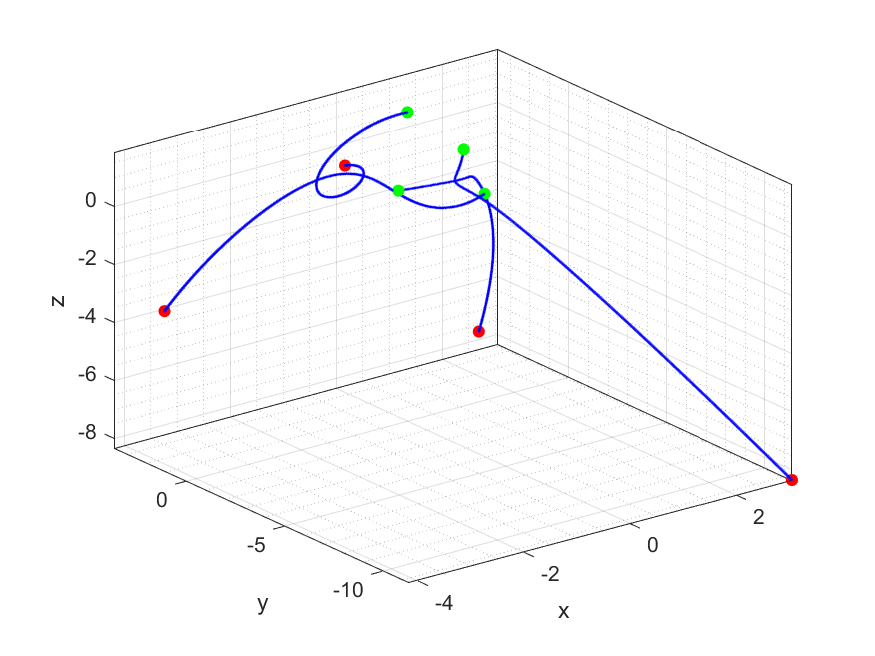
\includegraphics[width=\textwidth]{figures/4body.png}
        \caption{$N=4$}
        \label{fig:y equals x}
    \end{subfigure}
    \hfill
    \begin{subfigure}[b]{0.6\textwidth}
        \centering
        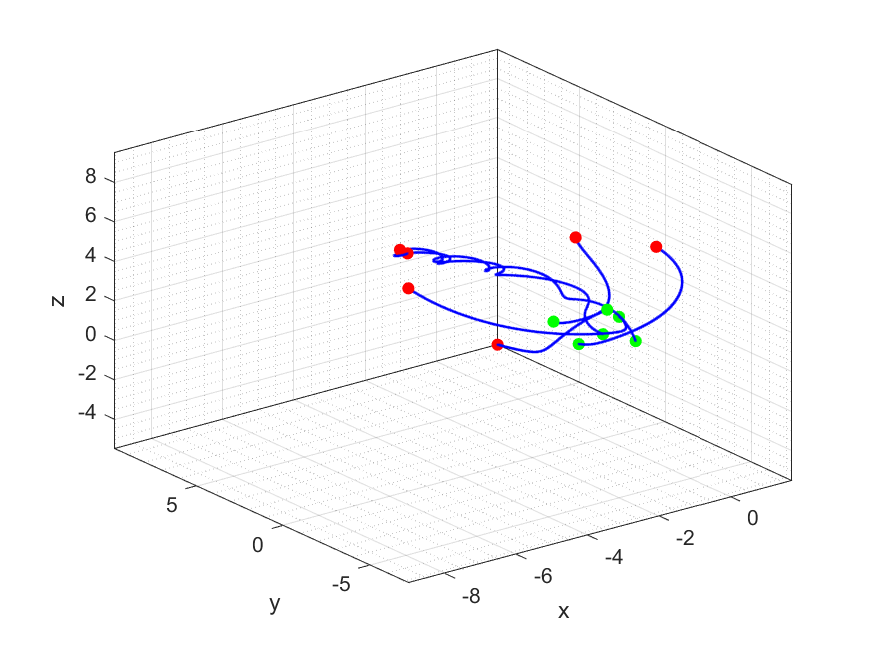
\includegraphics[width=\textwidth]{figures/6body.png}
        \caption{$N=6$}
        \label{fig:three sin x}
    \end{subfigure}
    \hfill
    \begin{subfigure}[b]{0.6\textwidth}
        \centering
        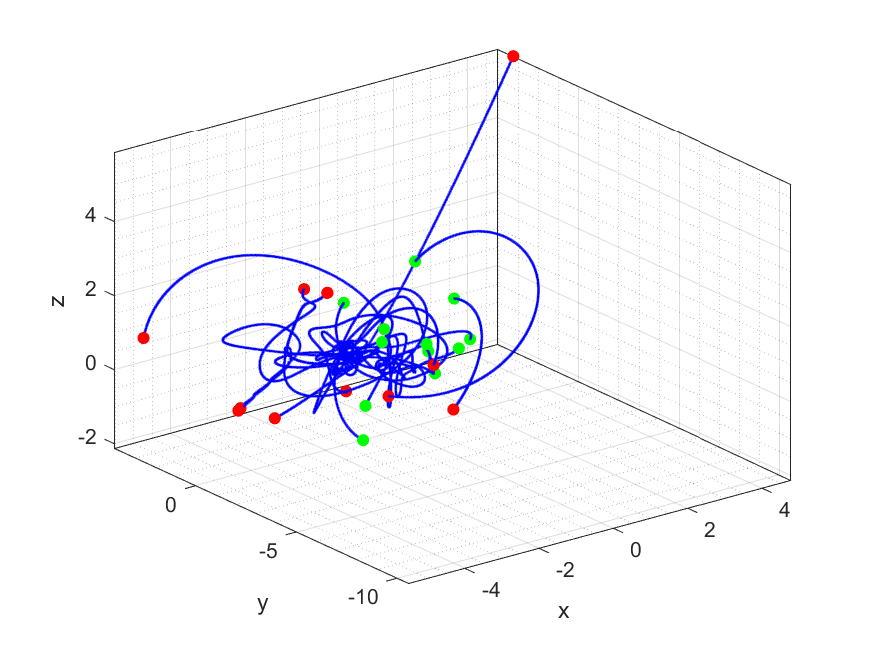
\includegraphics[width=\textwidth]{figures/12body.png}
        \caption{$N=12$}
        \label{12}
    \end{subfigure}
       \caption{Problem $N$-teles}
       \label{Nbody}
\end{figure}



\section{Problem treh teles}

Najpogosteje raziskan problem $N$-teles je problem treh teles, tj. $N=3$.
S problemom treh teles se matematiki ukvarjajo že od Newtonovega prvotnega raziskovanja tega problema dalje,
z željo po razumevanju gibanja sistema Sonce-Zemlja-Luna.
Prvi je pod tem imenom problem objavil Jean le Rond d'Alembert leta 1747.

\subsection{Posebni primeri problema treh teles}

Leonhard Euler je leta 1767 odkril tri družine rešitev pri katerih so tri telesa ves čas gibanja kolinearna
in se gibljejo okoli skupnega masnega središča.
Rešitev je zelo nestabilna, lahko jo porušijo že majhne pertubacije.
Na sliki \ref{Euler} je prikazano gibanje treh teles glede na Eulerjevo kolinearno rešitev.
\begin{figure}[H]
    \centering
    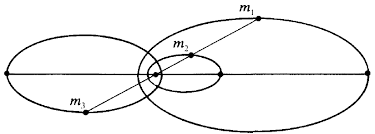
\includegraphics[width=\textwidth]{figures/euler_slika.png}
    \caption{Eulerjeva rešitev}
    \label{Euler}
\end{figure}

Leta 1772 je Lagrange odkril novo družino rešitev, kjer telesa med gibanjem ves čas tvorijo
oglišča enakostraničnega trikotnika.
Začetne pogoje izberemo kot v \cite{James} in določimo:
\begin{align*}
    x_1 &=-0.0833, & y_1&= 0.7217, & z_1 &=0, \\
    x_2 &= -0.5833, & y_2 &= -0.1443, & z_2 &=0, \\
    x_3&=0.4167, & y_3&=-0.1443, &  z_3&=0
\end{align*}
in $m = (1,1,1)$. Dobimo simulacijo na sliki \ref{Lagrange}.
\begin{figure}[H]
    \centering
    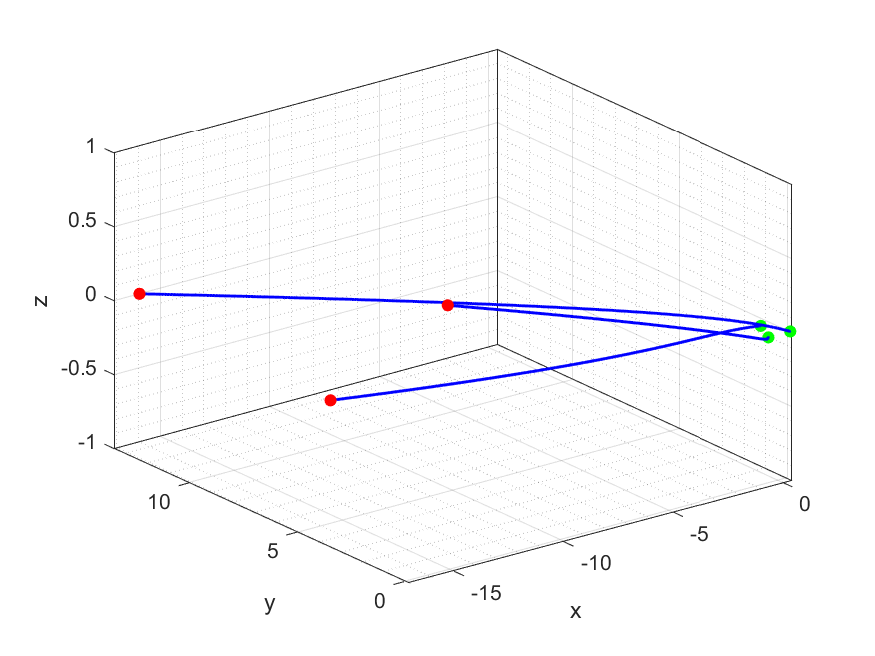
\includegraphics[width=\textwidth]{figures/Lagrange.png}
    \caption{Lagrangeva rešitev z enakostraničnim trikotnikom}
    \label{Lagrange}
\end{figure}

Še eno znano rešitev problema treh teles je leta 1993 odkril Chris Moore, in sicer problem pri katerem
se tri telesa periodično gibljejo po obliki osmice, 
to rešitev pa sta leta 2000 potrdila še Alain Chenciner in Richard Montgomery.
Za razliko od prejšnjih dveh primerov je ta rešitev stabilna.
Začetne pogoje v tem primeru povzamemo po \cite{James}. Definiramo: 
\begin{align*}
    x_1&=-0.97000436, &  y_1&=0.24308753, & z_1&=0, \\
    x_2&=0.97000436, & y_2&=-0.24308753, & z_2&=0, \\
    x_3&=0, & y_3&=0, & z_3&=0
\end{align*}
in $m = (1, 1, 1)$. Dobimo simulacijo na sliki \ref{osmica}.
\begin{figure}[H]
    \centering
    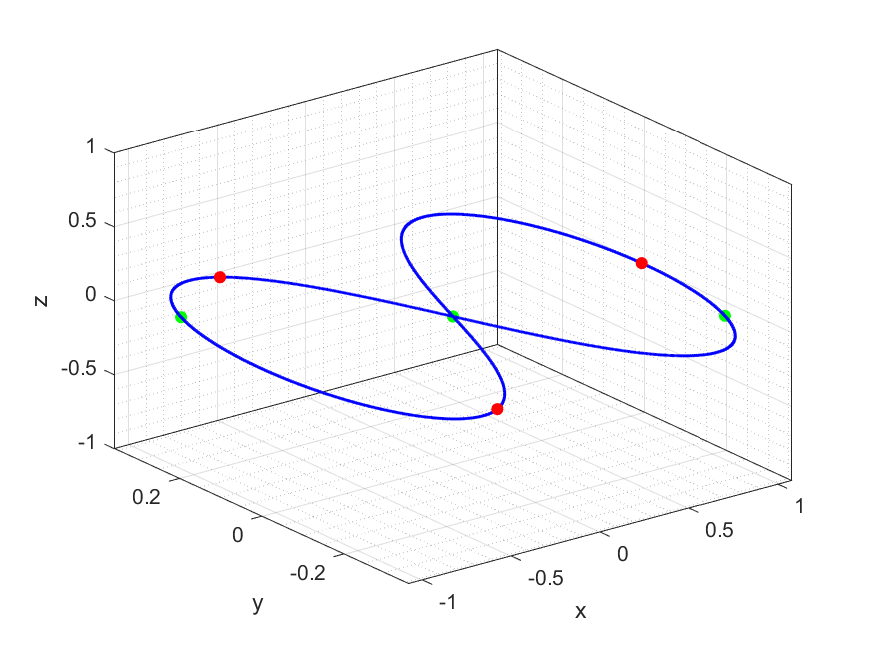
\includegraphics[width=\textwidth]{figures/osmica.png}
    \caption{Problem treh teles-gibanje po osmici}
    \label{osmica}
\end{figure}



\section{Zaključek}
Problem $N$-teles je znan matematično-fizikalni problem s katerim se znanstveniki ukvarjajo že vrsto let.
Glavna motivacija zanj je želja po razumevanju gibanja nebesnih teles, še posebej specifike gibanja 
Sonce-Zemlja-Luna. Problem ima mnoge implikacije tudi v drugih znanostih, kot na primer simulacije proteinov 
v strukturni biologiji, preučevanje kemijskih vezi in molekul, v statistiki in strojnem učenju.

\begin{thebibliography}{1}
 
    \bibitem{Cohan}
    A.~Cohan, \emph{A Figure Eight And other Interesting Solutions to the N-Body Problem},
    Department of mathematics, University of Washington, Washington, June 2012.

    \bibitem{James}
    J.D.~M.~James, \emph{Celestial Mechanics Note Set 3: General Three
    Body Problem and the Orbital Configurations of
    Euler and Lagrange}, 
    v: January 1, 2007, [26.10.2022], dostopno na \url{https://cosweb1.fau.edu/~jmirelesjames/hw3Notes.pdf}.
    
    \bibitem{Hom}
    K.~Mack, \emph{Homework No. 7},
    v: December 1, 2017, [26.10.2022], dostopno na \url{https://mackkv.github.io/files/ee520-hw7.pdf}.
    \bibitem{Mocz}
    P.~Mocz, \emph{Create Your Own N-body Simulation (With Matlab)},
    v: September 14, 2020, [26.10.2022], dostopno na \url{https://medium.com/swlh/create-your-own-n-body-simulation-with-matlab-22344954228e}.
    \bibitem{Nbody}
    \emph{N-body problem},
    v: March, 2017, [26.10.2022], dostopno na \url{https://en.wikipedia.org/wiki/N-body_problem}
    \bibitem{3body}
    \emph{Three-body problem},
    v: March, 2017, [26.10.2022], dostopno na \url{https://en.wikipedia.org/wiki/Three-body_problem#Special-case_solutions}
    \bibitem{Spec}
    T.~Guan, \emph{Special cases of the three body problem}, 
    v: dostopno na \url{http://inside.mines.edu/fs_home/tohno/teaching/PH505_2011/Paper_TianyuanGuan.pdf}
    
\end{thebibliography}


\end{document}